%%%%%%%%%%%%%%%%%%%%%%%%%%%%%%%%%
%% Ersetzen Sie in den folgenden Zeilen die entsprechenden -Texte-
%% mit den richtigen Werten.
\documentclass[course=erap]{aspdoc}
\newcommand{\theGroup}{155} % Beispiel: 42
\newcommand{\theNumber}{A501} % Beispiel: A123
\author{Mete Polat \and Jonas Hübotter \and Simon Martin Bohnen}
\date{Sommersemester 2019} % Beispiel: Wintersemester 2018/19
%%%%%%%%%%%

\usepackage{amssymb}
\usepackage{icomma}
\usepackage{hyperref}
\usepackage{tabularx}
\usepackage{pgfplots}
\usepackage{varwidth}
\usepackage[block=ragged]{biblatex}
\usepackage{multicol}
\pgfplotsset{width=12cm,compat=1.9}
\addbibresource{bib/Literatur.bib}
\renewcommand*{\bibfont}{\small}

% Diese Zeile bitte -nicht- aendern.
\title{Gruppe \theGroup{} -- Abgabe zu Aufgabe \theNumber}

\begin{document}
\maketitle

\section{Einleitung}

Im Folgenden wird die symmetrische Blockchiffre RC5 sowie die Implementierung dieser beschrieben. Zunächst wird der Algorithmus näher spezifiziert und auf dessen Sicherheit eingegangen. Daraufhin werden Aspekte der Lösungsfindung besprochen und der Implementierung dokumentiert. Abschließend wird die Implementierung gegen eine Referenzimplementierung getestet und die Performanz analysiert.

\section{Problemstellung und Spezifikation}

\subsection{RC5-16/16/b}

\subsubsection{Schlüsselerweiterung mit P und Q}

RC5 ist rundenbasiert, weshalb zunächst aus dem gegebenen Schlüssel mehrere Rundenschlüssel erzeugt werden. Für den Schritt der Schlüsselexpansion von RC5 werden die beiden ungeraden Ganzzahlen $P$ und $Q$ benötigt. Diese sind jeweils für eine gegebene Blockgröße von RC5 konstant. Für das von uns implementierte RC5-16/16/b gilt:

\begin{multicols}{2}
\noindent
\begin{align*}
P &= Odd((e - 2) \cdot 2^{16}) \\
  &= Odd(0,71828 \cdot 65.536) \\
  &= Odd(47.073,19808) \\
  &= 47.073 = 0xb7e1
\end{align*}
\begin{align*}
Q &= Odd((\phi - 1) \cdot 2^{16}) \\
  &= Odd(0,61803 \cdot 65.536) \\
  &= Odd(40.503,21408) \\
  &= 40.503 = 0x9e37
\end{align*}
\end{multicols}

\subsubsection{Sicherheit}
\label{sec:Sicherheit}

Durch die Parametrisierung von RC5-$w$/$r$/$b$ hat die Chiffre eine variable Halbblockgröße $w$, Rundenanzahl $r$ und Schlüssellänge $b$ \cite[p.2]{rc5rev}. Zusammen mit dem Betriebsmodus bestimmen diese Parameter die Sicherheit von RC5.

\paragraph{Schlüssellänge} So wie im Allgemeinen bei Blockchiffren ist auch bei RC5 die Sicherheit der Chiffre stark von der gewählten Schlüssellänge abhängig. Der Parameter $b \in \{k \in \mathbb{N}_0 \colon k \leq 255\}$ gibt die Länge des Schlüssels in Bytes an \cite[p.3]{rc5rev}. Die Länge der erweiterten Schlüsseltabelle in Bits ergibt sich durch $2^{(2r + 2)w}$ \cite[p.2]{rc5rev}. Der Aufwand für eine \textit{erschöpfende Suche} ist damit $min\{2^{8b}, 2^{(2r + 2)w}\}$ \cite[p.29]{kaliski+yin}. Für RC5-16/16/b ist damit der Aufwand einer erschöpfenden Suche allein von $b$ abhängig, solange $b < 68$ gilt.\bigbreak

Das Bundesamt für Sicherheit in der Informationstechnik (BSI) schlägt für Blockchiffren wie RC5 eine minimale Schlüssellänge von $128$ Bits vor \cite[p.21]{bsi}.

\paragraph{Betriebsmodus} Ist der durch den Betriebsmodus generierte Ciphertext nicht pseudorandom --- resultieren äquivalente Plaintext-Blöcke beispielsweise in äquivalenten Ciphertext-Blöcken ---, dann enthält der Ciphertext Informationen zur Struktur des Plaintextes \cite[p.22]{bsi}. In diesem Fall können Teile des Plaintextes durch \textit{Häufigkeitsanalyse} rekonstruiert \cite[p.22]{bsi}, oder sogar der verwendete Schlüssel durch einen \textit{Codebook Attack} gewonnen werden \cite[p.2]{elbaz}.\bigbreak

Sichere Modi sind beispielsweise \textit{Cipher Block Chaining (CBC)} und der \textit{Counter Mode (CTR)}, da dort der $n$-te Chiphertext-Block nicht nur von dem $n$-ten Plaintext-Block und dem genutzten Schlüssel abhängt, sondern zudem noch von einem weiteren Wert, wie dem $(n-1)$-ten Ciphertext-Block oder einem Zähler \cite[p.22]{bsi}.

\paragraph{Rundenanzahl} Nach Kaliski und Yin werden für eine \textit{differenzielle Kryptoanalyse} von RC5-32/16/b entweder $2^{61}$ selbst gewählte Plaintexte oder $2^{63}$ bekannte Plaintexte benötigt. Ein solcher Angriff auf ein $16$-rundiges RC5 ist damit überaus unwahrscheinlich. Da die Anzahl der möglichen Plaintexte bei dieser Konfiguration von RC5 jedoch bei $2^{64}$ liegt, kann ein solcher Angriff nicht theoretisch ausgeschlossen werden \cite[p.6]{kaliski+yin}. Weiterhin sei eine \textit{lineare Kryptoanalyse von RC5} nur bei einer sehr geringen Rundenzahl von RC5 effektiv \cite[p.28]{kaliski+yin}.\bigbreak

Knudsen und Meier zeigen zwar, dass die Komplexität des von Kaliski und Yin vorgeschlagenen differenziellen Angriffs um einen Faktor von bis zu $512$ reduziert werden kann \cite[p.2]{knudsen+meier}, allerdings bleibt ein solcher Angriff damit weiterhin sehr unwahrscheinlich. Zudem wurde gezeigt, dass für bestimmte Teile des Schlüsselraums die differentiellen Kryptoanalysen weiter verbessert werden können \cite[p.13]{knudsen+meier}. Für einen effektiven Angriff sind dennoch entweder zu wenige Schlüssel betroffen oder die Anzahl der benötigten Plaintexte ist weiterhin zu hoch. Ähnliches konnte Heys für lineare Kryptoanalyse zeigen \cite[p.5]{heys}.

\paragraph{Blockgröße} Durch die $32$ Bit Blockgröße von RC5-16/16/b ist die Komplexität eines \textit{generischen Angriffs} durch $2^{32}$ nach oben beschränkt. Bellare et al. zeigen für CBC, dass die Unsicherheit eines generischen Angriffs durch
\[
    \epsilon \geq \left(\frac{\mu^2}{l^2} - \frac{\mu}{l}\right) \cdot \frac{1}{2^l}
\]
gegeben ist, wobei $l = 2w$ der Blockgröße, $\mu = q \cdot l$ der Länge der verarbeiteten Plaintexte und $q$ der Anzahl der verarbeiteten Blöcke entspricht \cite[p.5;24]{bellare}. Damit kann eine untere Schranke $\epsilon$ für die Erfolgswahrscheinlichkeit eines solchen Angriffs durch
\[
    \epsilon \geq \frac{q^2}{2^l}
\]
abgeschätzt werden. Die minimale Erfolgswahrscheinlichkeit eines generischen Angriffs auf eine 32-Bit Blockchiffre ist somit $2^{-32}$. Aus diesem Grund eignen sich $32$-Bit Blockchiffren im Allgemeinen und RC5-16/16/b im Speziellen nicht für die Verschlüsselung von großen Datenmengen. Die RC5-Chiffre kann damit bei für die Anwendung ausreichend großer Blockgröße und Rundenanzahl, $b >= 16$ und Nutzung eines geeigneten Betriebsmodus als sicher gelten. RC5-16/16/b eignet sich in der Regel lediglich zur Verschlüsselung von kleinen Datenmengen für die $q \ll 2^{16} = 2^{l/2}$ gilt.

\subsection{Feistelchiffren}

Die folgende allgemeine Darstellung von Feistelchiffren soll auf klassische (auch ausgewogene) Feistelchiffren begrenzt werden. Wie für RC5, gilt für klassische Feistelchiffren, dass die Längen der beiden Halbblöcke eines Blocks gleich sein müssen. Zudem wird sich auf das für die umkehrbare Verknüpfung von zwei Halbblöcken übliche $\oplus$ (XOR) beschränkt.

\subsubsection{Einrundige Feistelnetzwerke}

Eine Feistelchiffre ist eine rundenbasierte Blockchiffre, die nach der Art eines Feistelnetzwerks aufgebaut ist. Sei
\[
    F_n := \{f \mid f \colon \{0, 1\}^n \to \{0, 1\}^n\}
\]
die Famile der Rundenfunktionen. Zunächst soll ein klassisches einrundiges Feistelnetzwerk $\Psi$ betrachtet werden. Dieses wird definiert durch eine beliebige Abbildung $f \in F_n$ und eine umkehrbare Bitoperation --- durch obige Einschränkung der Allgemeinheit $\oplus$.
\[
    \Psi(f) \colon \{0, 1\}^{2n} \to \{0, 1\}^{2n} \colon [L, R] \mapsto [S, T] \Leftrightarrow
        \begin{cases}
            S = R \\
            T = L \oplus f(R) \\
        \end{cases}
\]
für $\forall(L, R) \in (\{0, 1\}^n)^2$ \cite[p.11]{nachef} (siehe Abbildung 1). Wichtig für jede Verschlüsselung ist Bijektivität, damit jedem Codewort eine eindeutige Plaintext-Nachricht zugeordnet werden kann. $\Psi(f)$ ist unabhängig von $f \in F_n$ eine Permutation, d.h. $f$ selbst muss nicht bijektiv sein \cite[p.12]{nachef}. Aus der Definition von $\Psi(f)$ ergibt sich ihr Inverses als
\[
    \Psi(f)^{-1} = \sigma \circ \Psi(f) \circ \sigma
\]
mit $\sigma$ definiert als $\sigma([L, R]) = [R, L]$ für $L, R \in \{0, 1\}^n$, der Vertauschung beider Halbblöcke \cite[p.12]{nachef} (siehe Abbildung 2).

\subsubsection{r-rundige Feistelnetzwerke}

Üblicherweise werden Feistelnetzwerke in mehreren Runden angewendet. Im Allgemeinen ist ein klassisches Feistelnetzwerk mit $r \geq 1$ Runden und $f_1, f_2, ..., f_r \in F_n$ Rundenfunktionen definiert durch
\[
    \Psi^r(f_1, ..., f_r) = \Psi(f_r) \circ ... \circ \Psi(f_2) \circ \Psi(f_1).
\]\cite[p.12]{nachef} (siehe Abbildung 3)

\begin{multicols}{2}
{
\begin{center}
    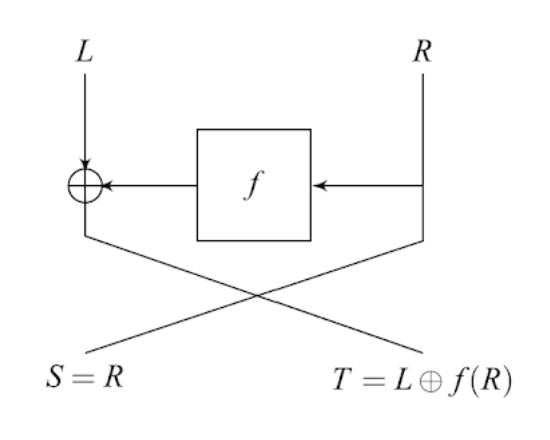
\includegraphics[scale=1]{img/1_round_feistel_cipher_enc.png}\break
    Abbildung 1: Einrundiges Feistelnetzwerk \cite[Fig. 2.1]{nachef}\\
    \vspace{5mm}
    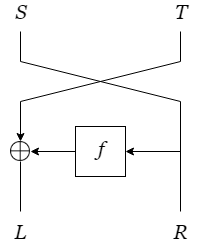
\includegraphics[scale=0.4]{img/1_round_feistel_cipher_dec.png}\break
    Abbildung 2: Inverses eines einrundigen Feistelnetzwerks\bigbreak
\end{center}
}
{
\begin{center}
    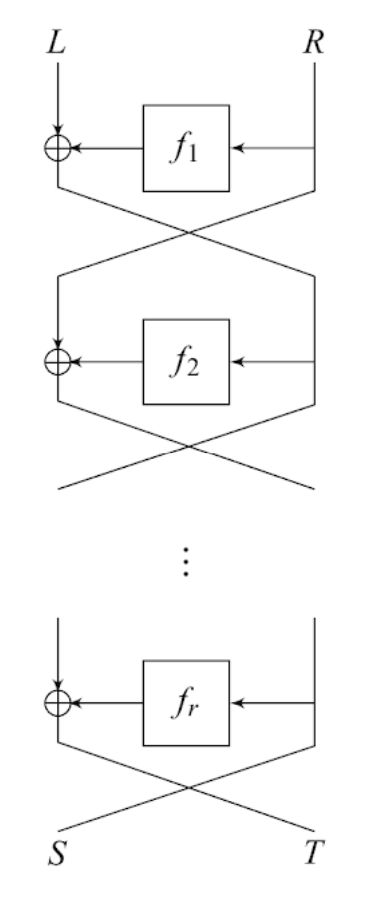
\includegraphics[scale=1]{img/r_round_feistel_cipher_enc.png}\break
    Abbildung 3: r-rundiges Feistelnetzwerk \cite[Fig. 2.2]{nachef}
\end{center}
}
\end{multicols}

Da ein einrundiges Feistelnetzwerk eine Permutation über $\{0,1\}^{2n}$ ist, sind auch $r$-rundige Feistelnetzwerke Permutationen. Weiterhin ist das Inverse eines $r$-rundigen Feistelnetzwerks die Komposition der Inversen der einzelnen Runden \cite[p.13]{nachef}.
\begin{align*}
    (\Psi^r(f_1, ..., f_r))^{-1} &= \sigma \circ \Psi(f_1) \circ \sigma \circ ... \circ \sigma \circ \Psi(f_r) \circ \sigma \\
                                 &= \sigma \circ \Psi^r(f_r, ..., f_1) \circ \sigma
\end{align*} Eine Feistelchiffre ist nun ein spezielles Feistelnetzwerk, dessen Rundenfunktionen von einem Rundenschlüssel aus dem Schlüsselraum $K$ abhängen.
Seien die Rundenschlüssel $(k_1, ..., k_r) \in K^r$ und die Familie der Rundenfunktionen
\[
    F_{n, K} := \{f_k \mid k \in K, f_k \colon \{0, 1\}^n \to \{0, 1\}^n\}.
\]
Dann ist eine Feistelchiffre das Feistelnetzwerk $\Psi^r(f_{k_1},...,f_{k_r})$. Also die $r$-rundige Permutation von der Nachricht $\{0, 1\}^{2n}$ in Abhängigkeit vom Schlüssel $(k_1, ..., k_r)$ \cite[p.14]{nachef}.

\subsubsection{RC5 als Feistelchiffre}

RC5 baut zu Beginn die erweiterte Schlüsseltabelle $S$ auf, die aus $2r + 2$ Schlüsseln besteht und von $K$ abhängt. Seien $\Sigma := (S_2, S_3, ..., S_{2r+1}) = (\Sigma_0, \Sigma_1, ..., \Sigma_{2r-1})$ mit $|\Sigma| = 2r$ die Schlüssel aus der erweiterten Schlüsseltabelle, die während der Runden von RC5 zum Verschlüsseln benutzt werden --- $S_0$ und $S_1$ werden für das Key-Whitening genutzt. Zudem sei $(g_{\Sigma_0}, g_{\Sigma_1}, ..., g_{\Sigma_{2r-1}})$ definiert durch
\begin{align*}
    g_k \colon &\{0, 1\}^w \times \{0, 1\}^w \to \{0, 1\}^w \colon \\
               &(\tau, R) \mapsto (\tau \lll R) + k
\end{align*}
mit $\tau = L \oplus R$, $k \in \Sigma$ und $L, R \in \{0, 1\}^w$ wobei $x \lll y$ die Linksrotation von $x$ um $y$ Bits angibt. Dann zeigt die folgende Tabelle die Zusammenhänge von RC5 und Feistelchiffren.

\begin{center}
 \begin{tabular}{c|c}
 RC5 & Feistelchiffre \\
 \hline
 $r$ & $2r$ \\
 $w$ & $n$ \\
 $\Sigma$ & $K^{2r}$ \\
 $(g_{\Sigma_0}, g_{\Sigma_1}, ..., g_{\Sigma_{2r-1}})$ & $(f_{k_1}, ..., f_{k_{2r}}) \in F^{2r}_{n, K}$ \\
\end{tabular}
\end{center}

Die Reihenfolge der Anwendung der umkehrbaren Bitoperation ($\oplus$) und der Rundenfunktion unterscheidet sich leicht zwischen RC5 und einer allgemeinen klassischen Feistelchiffre. Dieser Unterschied soll in der folgenden Abbildung skizziert werden.

\begin{samepage}
\begin{center}
    \includegraphics[scale=0.5]{img/rc5_feistel_cipher.png}\break
    Abbildung 4: Links eine Runde einer Feistelchiffre, rechts eine Runde (zwei Halbrunden) von RC5
\end{center}
\end{samepage}

wobei $r$ die aktuelle Runde angibt. Wie dargestellt, ist eine Halbrunde von RC5 im Aufbau ähnlich zu einer Runde einer Feistelchiffre.\bigbreak

Durch den leicht modifizierten Aufbau einer Feistelchiffre in RC5, verändert sich bei RC5 die Berechnung der Inversen. Für eine RC5-Runde gilt
\[
    RC5_{r, \Sigma} \colon \{0, 1\}^{2w} \to \{0, 1\}^{2w} \colon [L, R] \mapsto [S, T] \Leftrightarrow
        \begin{cases}
            S = ((L \oplus R) \lll R) + \Sigma_{2r-2} \\
            T = ((R \oplus S) \lll S) + \Sigma_{2r-1} \\
        \end{cases}.
\]
Damit gilt für die Berechnung der Inversen von einer RC5-Runde
\[
    RC5_{r, \Sigma}^{-1} \colon \{0, 1\}^{2w} \to \{0, 1\}^{2w} \colon [S, T] \mapsto [L, R] \Leftrightarrow
        \begin{cases}
            L = ((S - \Sigma_{2r-2}) \ggg R) \oplus R \\
            R = ((T - \Sigma_{2r-1}) \ggg S) \oplus S \\
        \end{cases}
\]
für $\forall(S, T) \in (\{0, 1\}^w)^2$ wobei $x \ggg y$ die Rechtsrotation von $x$ um $y$ Bits angibt.

\subsection{PKCS\#7-Padding}

Da eine Blockchiffre nur Nachrichten vollständig verschlüsseln kann, die restfrei in Blöcke geteilt werden können, muss die Länge dieser Nachrichten zunächst auf ein Vielfaches der Blockgröße erweitert werden. Diese Erweiterung wird im Allgemeinen als Padding bezeichnet.\bigbreak

Das PKCS\#7-Padding ist eine Form der Erweiterung des Plaintextes auf ein Vielfaches der Blocklänge und soll im Folgenden erläutert werden. Es sei $\Delta$ definiert als
\[
    \Delta = b - (l \bmod b)
\]
mit $b$ als der Länge eines Blocks und $l$ als der Länge des Plaintextes in Byte. Vor der Anwendung eines Verschlüsselungsalgorithmus, der als Länge des Inputs ein Vielfaches von $b$ Bytes erwartet, werden $\Delta$ Bytes jeweils mit dem Wert $\Delta$ an den Plaintext angefügt \cite[p.28]{rfc5652}.\bigbreak

Das heißt, dass der Input in Abhängigkeit von $b$ und $l$ um eine der folgenden Byte-Sequenzen erweitert wird:

\begin{samepage}
\begin{center}
\begin{varwidth}{\linewidth}
\begin{verbatim}
         01 -- if l mod b = b-1
      02 02 -- if l mod b = b-2
          .
          .
          .
b b ... b b -- if l mod b = 0
\end{verbatim}
\end{varwidth}
\end{center}
\end{samepage}

Nach dem Entschlüsseln des Codewortes, kann das Padding auf eindeutige Weise entfernt werden, da jeder Plaintext --- einschließlich jener, deren Länge selbst ein Vielfaches der Blockgröße ist --- vor der Verschlüsselung mit PKCS\#7-Padding erweitert wurde. Die Anzahl der zu entfernenden Bytes wird durch das letzte Byte des letzten Blocks angegeben. PKCS\#7-Padding ist wohldefiniert für $b < 256$ \cite[p.28]{rfc5652}.

\section{Lösungsfindung}

\subsection{Initialisierungsvektor}
\label{sec:Initialisierungsvektor}
Eine Herausforderung ist die Erzeugung und Speicherung des Initialisierungsvektors, der beim Cipher Block Chaining Mode benötigt wird. Es ist einerseits entscheidend, dass dieser nicht aus zuvor bekannten Informationen erzeugt wird, wie es zum Beispiel bei SSL 3.0 und TLS 1.0 der Fall war. Dort führte dies zu einer Schwäche, falls dem Angreifer zwei aufeinanderfolgende Ciphertext-Blöcke bekannt waren \cite{ssltls}. Andererseits ist eine ausreichende Länge wichtig, um einem Related-Key-Attack vorzubeugen, der zum Beispiel das WEP-Protokoll betraf \cite{wep}.\bigbreak

Aufgrund der Blocklänge bietet sich nur ein 32-Bit-Initialisierungsvektor an, der pseudozufällig generiert wird.
Eine Geheimhaltung des Initialisierungsvektors ist nicht erforderlich \cite[p.194]{appcrypt}, weshalb der Vektor am Ende der verschlüsselten Datei gespeichert und dort bei der Entschlüsselung wieder ausgelesen wird.

\subsection{Optimierung durch SIMD}
Eine Optimierung durch SIMD ist möglich und sinnvoll, wenn ein Algorithmus auf mehreren Datenblöcken die selbe Operation ohne Abhängigkeiten zwischen Blöcken ausführt. Bei RC5 und dem CBC-Mode werden jedoch häufig Abhängigkeiten verwendet, um statistischen Analysen, wie sie zum Beispiel beim ECB-Mode möglich sind, vorzubeugen.\bigbreak

Beim Key-Mixing hängt der nächste Rundenschlüssel beispielsweise direkt vom vorherigen ab, wodurch eine Parallelisierung unmöglich wird.
Ähnliches gilt für die Ver- und Entschlüsselung, da dort zur Erzeugung des nächsten Ciphertextblocks der vorherige benötigt wird. Die einzige mögliche Optimierung ist das gleichzeitige Laden mehrerer Rundenschlüssel oder Blöcke aus dem Speicher, um die Anzahl der Zugriffe zu minimieren. Beim CBC-Betriebsmodus ist nur ein Laden mehrerer Rundenschlüssel möglich. Wir verwenden ein XMM-Register, um 8 16-Bit-Rundenschlüssel gleichzeitig zu laden. Für die tatsächliche Verwendung müssen diese jedoch aus dem XMM-Register entnommen werden, da nur eine Runde gleichzeitig berechnet werden kann.\bigbreak

Beim Counter-Betriebsmodus ist eine Optimierung durch SIMD möglich. Da der Counter leicht für mehrere Blöcke berechnet werden kann und die Verschlüsselung der Blöcke nicht voneinander abhängt, kann diese auf 8 Blöcken parallel erfolgen, indem die linken und rechten Halbblöcke jeweils in ein XMM-Register geladen werden.

\section{Dokumentation der Implementierung}
Die hier bereitgestellte RC5-Implementierung kann zur sicheren Ver- und Entschlüsselung von kleinen Datenmengen genutzt werden.
Voraussetzung dafür, ist das Wählen eines geeigneten Schlüssels mit mindestens 16 Byte Länge (siehe
\hyperref[sec:Sicherheit]{2.1.2 Sicherheit}).
Es stehen die Betriebsmodi Cipher Block Chaining (CBC), Counter Mode (CTR) und der unsichere Electronic Codebook (ECB) zur Verfügung, wobei letztere effizienter sind.\bigbreak

Im Folgenden ist die Gebrauchsanweisung der RC5-Implementierung beschrieben:

\begin{samepage}
\begin{verbatim}
rc5 <command>

    enc [-m <mode>] [-v] <key> <inputFile> [<outputFile>]
    dec [-m <mode>] [-v] <key> <inputFile> [<outputFile>]
    test [<testId>]
    perf

where <mode> is one of:
    cbc, ctr, ecb
\end{verbatim}
\end{samepage}

Es kann entweder verschlüsselt oder entschlüsselt werden. Sofern keine Ausgabedatei angegeben ist, wird das Ergebnis in die Eingabedatei geschrieben. Der \texttt{test}-Command kann zur Überprüfung der Korrektheit verwendet werden. Die Performance lässt sich mit dem \texttt{perf}-Command messen.

\paragraph{Sicherheitshinweise} Solange der Rechner nicht während einer Ver-/Entschlüsselung in den Suspend-Modus versetzt wird, stellt unsere Implementierung sicher, dass der Schlüssel nicht durch Swapping auf die Festplatte geschrieben wird. Nach abgeschlossener Ver-/Entschlüsselung werden die sensiblen Daten aus dem Arbeitsspeicher entfernt. Allerdings ist es möglich, dass durch Swapping, Teile der zu verschlüsselnden/entschlüsselten Daten auf die Festplatte geschrieben wird. Eine Komprimierung des Schlüssels ist auf diese Weise zwar nicht möglich, dennoch ist es empfehlenswert, die Swap-Partition zu verschlüsseln.

\subsection{Struktur der Implementierung}

Die Implementierung ist in die folgenden sieben Module gegliedert:

\begin{center}
\begin{tabular}{ |c|m{11.2cm}| }
\hline
\texttt{rc5} & Enthält die Implementierung der RC5-Chiffre, sowie der Betriebsmodi CBC, CTR und ECB. \\
\hline
\texttt{test} & Enthält die Funktion zum Ausführen der Korrektheits-Tests. \\
\hline
\texttt{perf} & Enthält die Funktion zum Ausführen der Performance-Tests. \\
\hline
\texttt{key\_expansion} & Enthält die Implementierung zur Vorberechnung der Rundenschlüssel. \\
\hline
\texttt{enlighten} & Enthält die Implementierung für das Kopieren des BMP-Datei-Headers aus der ursprünglichen in die verschlüsselte Datei, damit diese durch ein Bildprogramm dargestellt werden kann. \\
\hline
\texttt{bufferio} & Enthält Library-Funktionen, die das Lesen aus und Schreiben in Dateien ermöglichen. \\
\hline
\texttt{references} & Enthält die RFC2040-Referenzimplementierung. \\
\hline
\end{tabular}
\end{center}

\subsection{Dateiaufbau}
Im Folgenden ist der Aufbau einer von der RC5-Implementierung verschlüsselten Datei aufgezeigt,
wobei der Initialisierungsvektor selbst nicht verschlüsselt wird.\\[1.5mm]
\begin{tabularx}{\textwidth}{|X|X|X|}
    \hline
    \centering Plaintext & \centering Padding & \centering\arraybackslash Initialisierungsvektor\\
    \hline
\end{tabularx}\\[1.5mm]
Siehe \hyperref[sec:Initialisierungsvektor]{3.1 Initialisierungsvektor} für dessen nähere
Beschreibung.

\subsection{Optimierungen}

\paragraph{Einmaliges Ausführen der Schlüsselexpansion} Ein bei gleicher Rundenanzahl und Blockgröße stets gleich bleibender Schritt bei der Ver- und Entschlüsselung ist die Schlüsselexpansion. Diese hängt nur von den Nothing-Up-My-Sleeve-Zahlen $P$ und $Q$ ab und muss daher im Voraus nur einmal berechnet werden. Die resultierenden Rundenschlüssel werden in der data-Section unseres Assemblerprogramms gespeichert, um sie beim Key-Mixing weiterzuverwenden. Der Code zur Schlüsselexpansion ist seperat in den Dateien \texttt{key\_expansion.c} und \texttt{key\_expansion.S} zu finden.

\paragraph{Laden der Rundenschlüssel in SSE-Register} Für jede Runde von RC5 werden zwei der $2r + 2$ Rundenschlüssel verwendet. Um die Anzahl der Speicherzugriffe zu minimieren, laden wir alle vier Runden acht neue 16-Bit Schlüssel in ein SSE-Register. Die Schlüssel werden daraufhin nacheinander in die niederwertigsten Bits rotiert und von dort zur Weiterverarbeitung in ein Standardregister geladen.

\section{Ergebnisse}

\subsection{Korrektheit}

Zur Überprüfung der Korrektheit haben wir die Ergebnisse unserer Implementierung mit denen einer Referenzimplementierung verglichen. Die Referenzimplementierung, die wir verwenden, ist in RFC2040 der IETF enthalten \cite{rfc2040}. Testfälle können mit dem \texttt{test}-Command ausgeführt werden.

\subsection{Performance}

\begin{center}
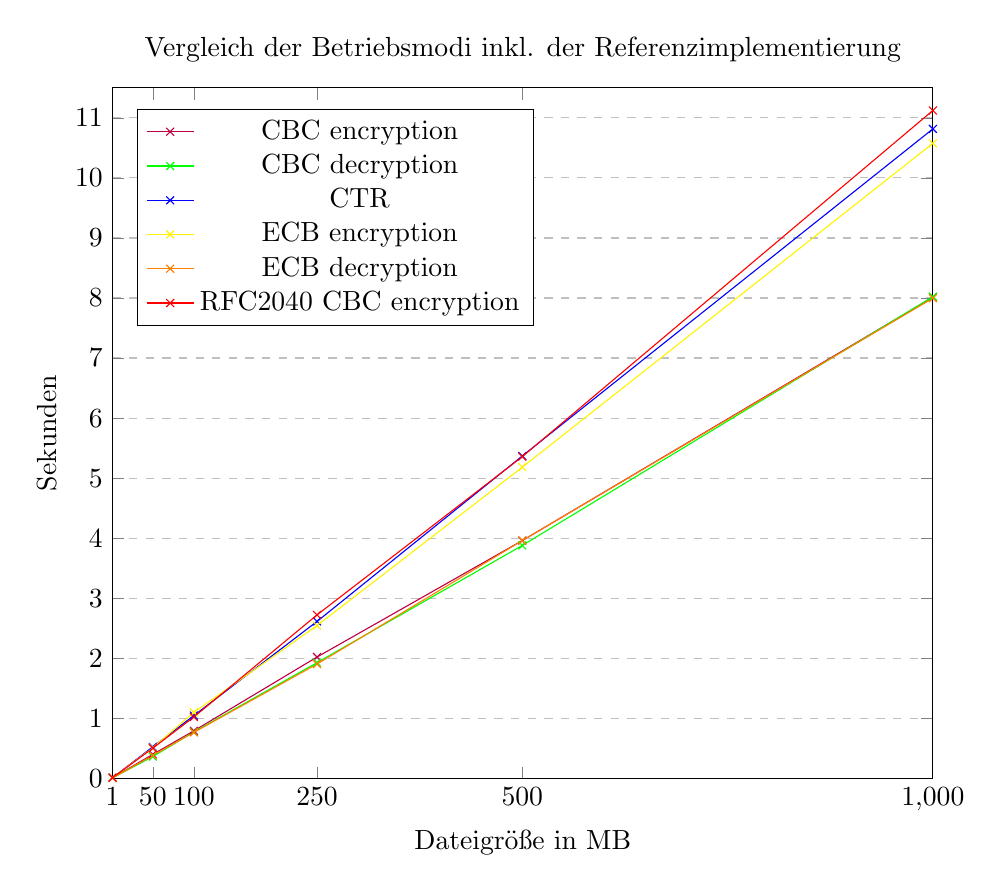
\begin{tikzpicture}
\begin{axis}[
    title={Vergleich der Betriebsmodi inkl. der Referenzimplementierung},
    xlabel={Dateigröße in MB},
    ylabel={Sekunden},
    xmin=1, xmax=1000,
    ymin=0, ymax=11.5,
    xtick={1,50,100, 250,500, 1000},
    ytick={0,1,2,3,4,5,6,7,8,9,10,11},
    legend pos=north west,
    legend entries={
    CBC encryption,
    CBC decryption,
    CTR,
    ECB encryption,
    ECB decryption,
    RFC2040 CBC encryption},
    ymajorgrids=true,
    grid style=dashed,
]
 
\addplot[
    color=purple,
    mark=x,
    ]
    coordinates {
    (1,0.008)(50,0.399)(100,0.791)(250,2.020)(500,3.960)(1000,8.012)
    };
\addplot[
   color=green,
   mark=x,
   ]
   coordinates {
   (1,0.007)(50,0.362)(100,0.772)(250,1.927)(500,3.879)(1000,8.022)
   };
\addplot[
   color=blue,
   mark=x,
   ]
   coordinates {
   (1,0.010)(50,0.524)(100,1.045)(250,2.613)(500,5.369)(1000,10.817)
   };
\addplot[
   color=yellow,
   mark=x,
   ]
   coordinates {
   (1,0.010)(50,0.509)(100,1.098)(250,2.544)(500,5.182)(1000,10.577)
   };
\addplot[
   color=orange,
   mark=x,
   ]
   coordinates {
   (1,0.007)(50,0.381)(100,0.765)(250,1.903)(500,3.960)(1000,7.997)
   };
\addplot[
   color=red,
   mark=x,
   ]
   coordinates {
   (1,0.010)(50,0.502)(100,1.021)(250,2.722)(500,5.358)(1000,11.124)
   };

\end{axis}
\end{tikzpicture}
\end{center}

Die Entschlüsselung mit dem CBC/ECB-Modus nutzt jeweils die Assemblerfunktion \texttt{rc5\_dec} und hat daher eine vergleichbare Laufzeit. Die Laufzeit der Verschlüsselung mit CBC ist ähnlich, da hier die zu \texttt{rc5\_dec} vergleichbare Assemblerfunktion \texttt{rc5\_enc} verwendet wird. Im Vergleich zur RFC2040-Implementierung
ist unsere Assemblerimplementierung um bis zu 26\% schneller.\bigbreak

Obwohl der Counter Mode sowie die Verschlüsselung im ECB-Modus mit SIMD-Instruktionen 8 Blöcke parallel verschlüsseln, sind sie deutlich langsamer als die übrigen Implementierungen. Die Konstruktion der Chiffre bedingt, dass die beiden Halblöcke jedes Blocks um den Wert des jeweils anderen Block rotiert werden müssen. Daher müssen die 8 Blöcke hier temporär aus den SSE-Registern geladen und einzeln rotiert werden.

\subsubsection{Vergleich des Assembler-Codes}

Für die Performance ist entscheidend, wie ein einzelner Block verschlüsselt wird. Im Folgenden ist der Code für eine Runde der RC5-Chiffre von unserer und der RFC2040-Implementierung zu sehen:

\begin{multicols}{2}

\noindent \textbf{Unsere Implementierung}

\begin{verbatim}
movd r11d, xmm0
pshufd xmm0, xmm0, 0b00111001
xor r9w, r10w
mov cl, r10b
rol r9w, cl
add r9w, r11w

shr r11d, 16
xor r10w, r9w
mov cl, r9b
rol r10w, cl
add r10w, r11w
add rax, 2
\end{verbatim}

\noindent \textbf{RFC2040-Implementierung}

\begin{verbatim}
mov    ecx,eax
xor    r8d,eax
add    rdx,0x4
and    ecx,0xf
rol    r8w,cl
add    r8w,WORD PTR [rdx-0x4]

mov    ecx,r8d
xor    eax,r8d
and    ecx,0xf
rol    ax,cl
add    ax,WORD PTR [rdx-0x2]

\end{verbatim}

\end{multicols}

\noindent Der Code ist in die Verschlüsselung des linken und des rechten Halbblocks aufgeteilt. Es ist deutlich zu erkennen, dass wir während der Verschlüsselung auf ein Laden der Rundenschlüssel verzichten. Stattdessen werden bei Bedarf acht neue Rundenschlüssel in \texttt{xmm0} geladen (hier nicht gezeigt). Bei der RFC2040-Implementierung wird jeder Rundenschlüssel einzeln aus dem Speicher geladen.

\section{Zusammenfassung}

Die RC5-Chiffre wurde mit unterschiedlichen Betriebsmodi erfolgreich implementiert und mit einer Referenzimplementierung verglichen. Es konnte gezeigt werden, dass der Einsatz von SSE-Registern zum Laden der Rundenschlüssel für eine deutliche Performance-Steigerung sorgt.\bigbreak

Aufgrund der Konstruktion der RC5-Chiffre eignet sich hingegen der Einsatz von SSE-Instruktionen für das paralelle Verschlüsseln mehrerer Blöcke in SSE-Registern nicht. Die Implementierung der Modi CTR und ECB könnte durch das parallele Verschlüsseln der Blöcke auf mehereren Hardware-Threads weiter beschleunigt werden. Weiterhin könnte das Anwendungsspektrum der Implementierung durch eine variable Wahl der Blockgröße und Rundenanzahl erweitert werden.

\newpage
\printbibliography

\end{document}

